\section{Fraxis gate}
\par Fraxis gate is the single qubit gate and can be defined as the $2\times 2$ unitary matrix $R(\bm{n})$ as the following,
$$\begin{aligned}
R(\bm{n})&=n_xX+n_yY+n_zZ
\end{aligned}$$
where $X$, $Y$, $Z$ are pauli matrices and parameters $\bm{n}=(n_x,n_y,n_x)^{ \mathrm{T} }$ satisfy the following :
$$\|\bm{n}\|^2=n_x^2+n_y^2+n_z^2=1
$$

\par Consider expressing one qubit quantum state on the Bloch sphere. It has been customary for a parameterized one-qubit gate to rotate the quantum state by a parameterized angle about some fixed axis. Fraxis gate breaks that convention and parameterizes the rotation axis by fixing the rotation angle to $\pi$ (See Figure \ref{fig:gate}).

On actual quantum processors, the number of quantum gates that can be used is limited, and various unitary operations are performed by combining gates available. Fraxis gate has to be also performed by those basic gates. For example, on ibmq\_montreal, fraxis gate is implemented as follows:
$$R(\bm{n})=R_z(\phi+\pi)\cdot\sqrt{X}\cdot R_z(\theta+\pi)\sqrt{X}\cdot R_z(\pi-\phi)$$
where
$$\theta=2\arctan\left(\frac{\sqrt{n_x^2+n_y^2}}{n_z}\right)$$
$$\phi=\arctan\left(\frac{n_y}{n_x}\right)$$

\begin{figure}[H]
    \centering
    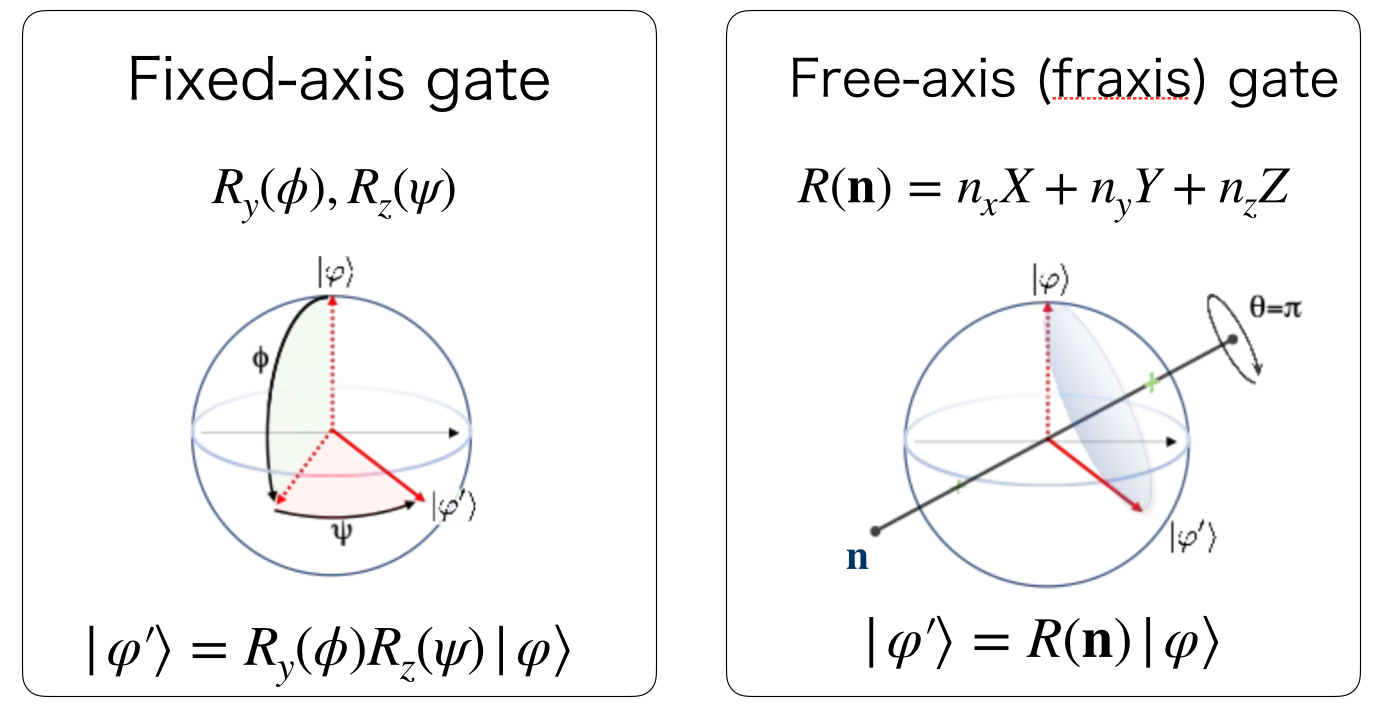
\includegraphics[keepaspectratio, scale=0.5]{preliminary/gate.png}
    \caption{Comparison of fraxis gate with the traditional parameterized gate. The pictures show how to rotate the quantum state $|\varphi\rangle$ to $|\varphi'\rangle$.}
    \label{fig:gate}
\end{figure}